\documentclass{article}
\usepackage{amsmath}
\documentclass{article}
\usepackage{listings}
\usepackage{xcolor}
\usepackage{matlab-prettifier}
\usepackage{graphicx}
\usepackage{fancyhdr}
\usepackage[sorting=none]{biblatex}
\usepackage[margin=1in]{geometry}
\usepackage{listings}
\usepackage[hidelinks]{hyperref}
\usepackage{xcolor}
\usepackage{xepersian}


\usepackage{subcaption}

\addbibresource{bibliography.bib}
\settextfont[Scale=1.2]{B-NAZANIN.TTF}
\setlatintextfont[Scale=1]{Times New Roman}
\renewcommand{\baselinestretch}{1.5}
\pagestyle{fancy}
\fancyhf{}
\rhead{پروژه چهارم درس داده‌کاوی }
\lhead{\thepage}
\rfoot{ آیلین نائب‌زاده}
\lfoot{99522185}
\renewcommand{\headrulewidth}{1pt}
\renewcommand{\footrulewidth}{1pt}

\begin{document}
\begin{titlepage}
\begin{center}

\includegraphics[width=0.4\textwidth]{IUSTLogo.png}\\
        
\LARGE
\textbf{دانشگاه علم و صنعت ایران}\\
\textbf{دانشکده مهندسی کامپیوتر}\\
        
\vfill
        
\huge
\textbf{عنوان: پروژه چهارم درس داده‌کاوی}\\
\textbf{رتبه‌بندی ویژگی‌های مؤثر در دسته‌بندی مجموعه داده‌ها}\\
\vfill
        
\LARGE
\textbf{نام و نام خانوادگی: آیلین نائب‌زاده }\\
\textbf{شماره دانشجویی: 99522185}\\
\textbf{نیم‌سال تحصیلی: پائیز 1402}\\
\textbf{مدرّس: دکتر حسین رحمانی}\\
\end{center}
\end{titlepage}


\tableofcontents
\newpage

\section{گام اول} 
در این پروژه هدف این است تا باتوجه به مجموعه داده برچسب‌ گذاری شده، ویژگی موجود را براساس میزان تاثیرگذاری رتبه‌بندی کنیم. فایل ورودی دارای 83 ستون و حدود 300000 ردیف می‌باشد. همچنین یک ستون بیانگر شماره ردیف با شروع از 1 و آخرین ستون نیز بیانگر برچسب نمونه‌ها می‌باشد که می‌تواند مقدار 0 یا 1 را داشته باشد.

بدلیل کمبود زمان و پیش بردن سریع‌تر مراحل خواسته‌شده به‌صورت موازی، گام‌های مورد نیاز برای حل پروژه، در دو فایل جداگانه به نام‌های \lr{DataMining - Prj4 - Supervised.ipyn} و \lr{DataMining - Prj4 - Unsupervised.ipynb} پیاده‌سازی شده‌اند.

\begin{figure}[ht]
        \centering
        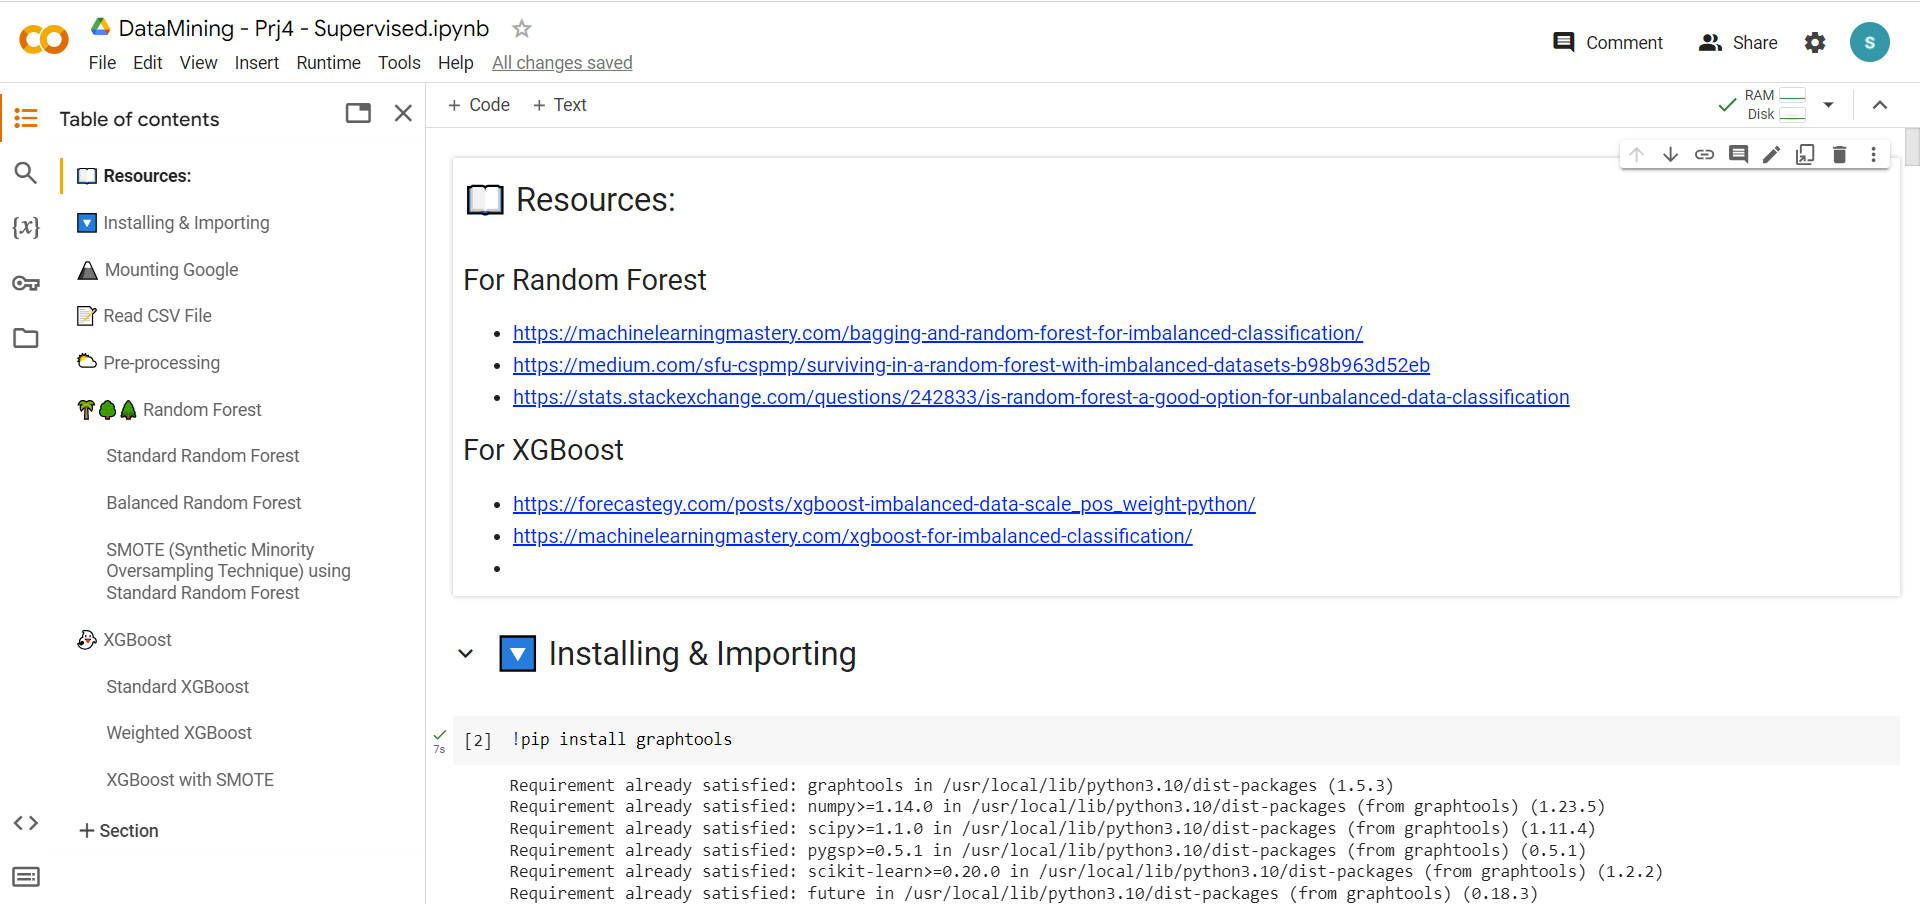
\includegraphics[width=0.6\textwidth]{im1-1-su.png}
        \caption{نمای کلی از پروژه با ناظر}
        \label{fig:fig1}
    \end{figure}
    
\begin{figure}[ht]
        \centering
        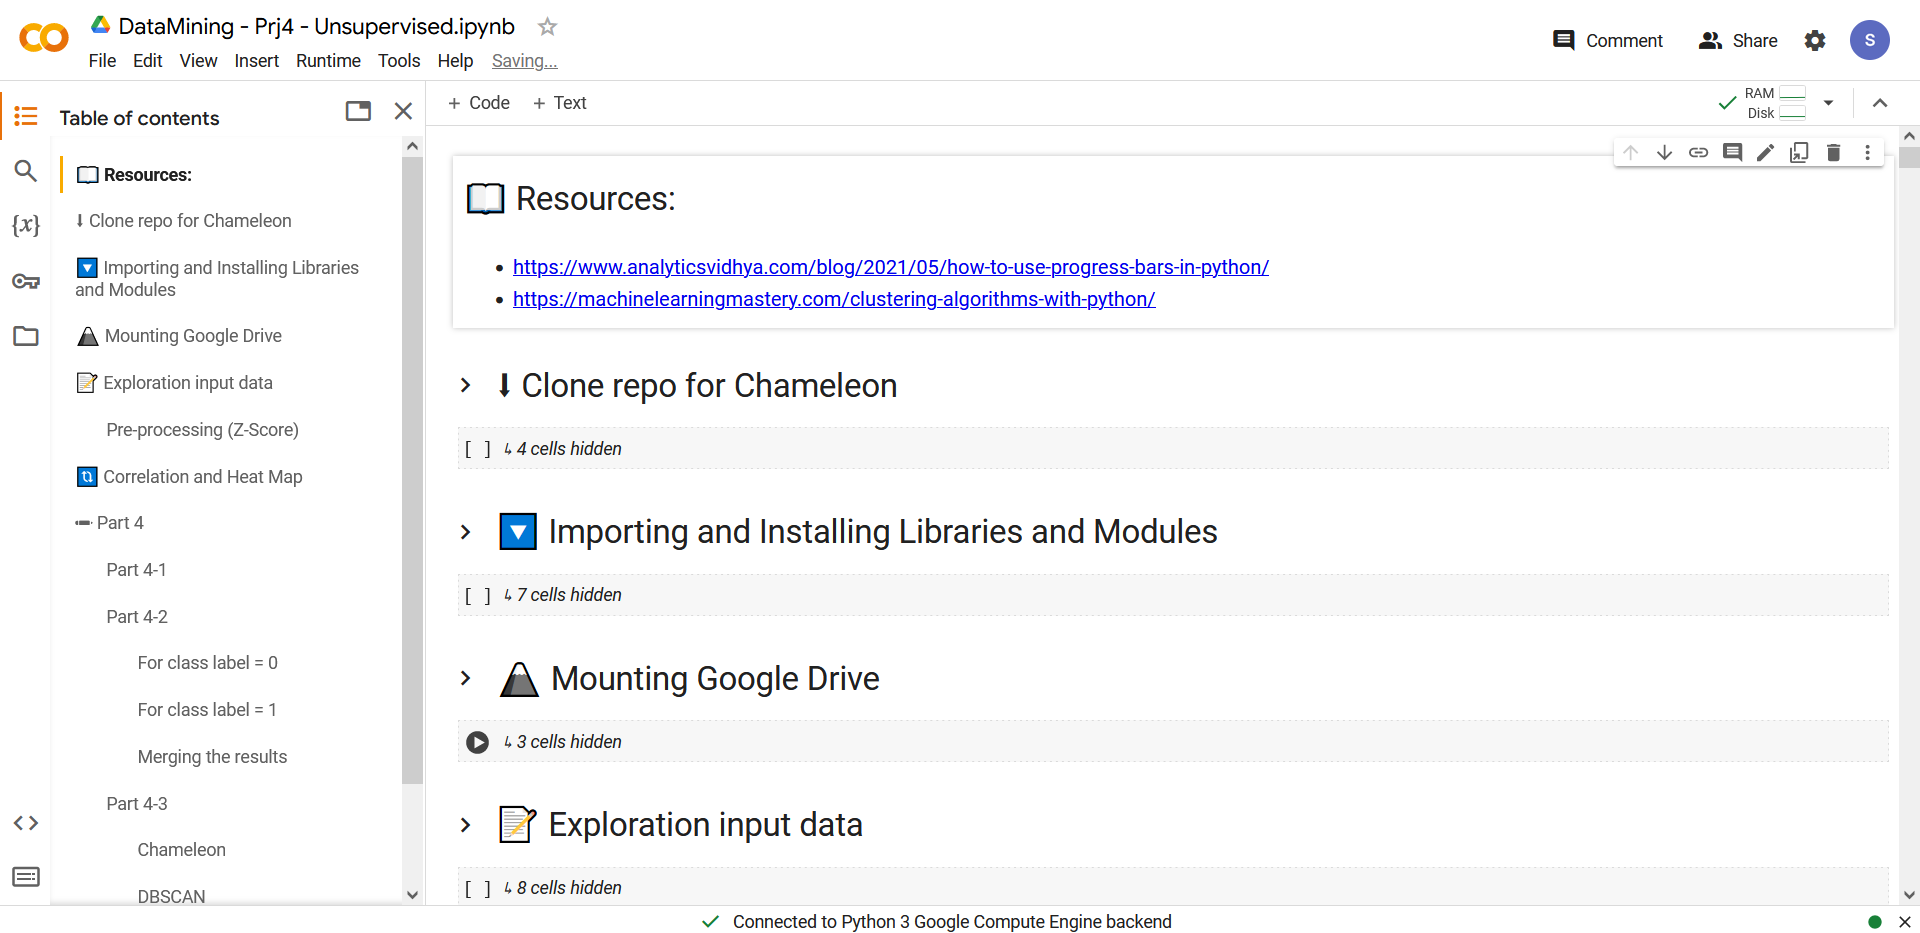
\includegraphics[width=0.6\textwidth]{img-1-un.png}
        \caption{نمای کلی از پروژه بدون ناظر}
        \label{fig:fig2}
    \end{figure}
    
در مرحله اول بااستفاده از کتابخانه \lr{pandas} و تابع \lr{read\_csv}، فایل‌های ورودی را به متغیرهایی از نوع \lr{dataframe} تبدیل می‌کنیم تا در قدم‌های بعدی راحت‌تر بتوانیم تحلیل‌های مورد نیاز را انجام بدهیم.
همچنین بااستفاده از توابع \lr{info()}، \lr{.head()} و \lr{.describe()} اطلاعات بیشتری نسبت به داده‌های موجود کسب می‌کنیم.

* خروجی تمامی مراحل ذکر شده بطور کامل در فایل‌های \lr{ipynb} موجود می‌باشند.
\newpage
\section{گام دوم}
طبق توضیحات ذکر شده در فایل پروژه به‌منظور پیش پردازش داده‌ها تنها کافی است عملیات نرمالایز را بر روی داده‌ها انجام دهیم.
البته همان‌گونه که در خروجی تابع \lr{.info()} می‌توانید مشاهده کنید، هیچ یک از ستون‌ها شامل مقادیر \lr{None} نمی‌باشد و همگی دارای 298714 مقدار غیر تهی می‌باشند.

حال به‌منظور انجام عملیات \lr{normalization} از تابع آماده \lr{StandardScaler()} موجود در کتابخانه \lr{sklearn.preprocessing} استفاده می‌کنیم. درواقع این تابع عملیات \lr{Z-Score} را بر روی ویژگی‌های گوناگون به‌طور جداگانه انجام می‌دهد.

البته به این نکته دقت شود که نیازی نیست که برروی ستون‌های اول و آخر مجموعه داده‌های ورودی نیز این عملیات انجام شود.
\begin{figure}[ht]
        \centering
        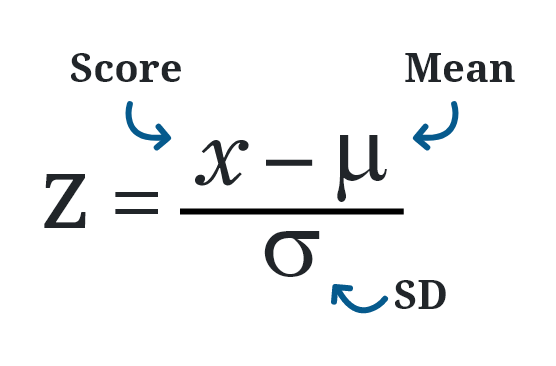
\includegraphics[width=0.6\textwidth]{Zscore_39.png}
        \caption{رابطه \lr{Z-Score}}
        \label{fig:fig3}
    \end{figure}
    
\newpage
\section{گام سوم}
در این مرحله همان‌طور که خواسته شده‌است، ماتریس همبستگی میان ویژگی‌های موجود را بدست می‌آوریم. برای محاسبه این ماتریس می‌توانیم از تابع آماده \lr{.corr()} که در کتابخانه \lr{pandas} موجود می‌باشد استفاده کنیم.

تصویر ماتریس نهایی را در شکل زیر می‌توانید مشاهده کنید.
\begin{figure}[ht]
        \centering
        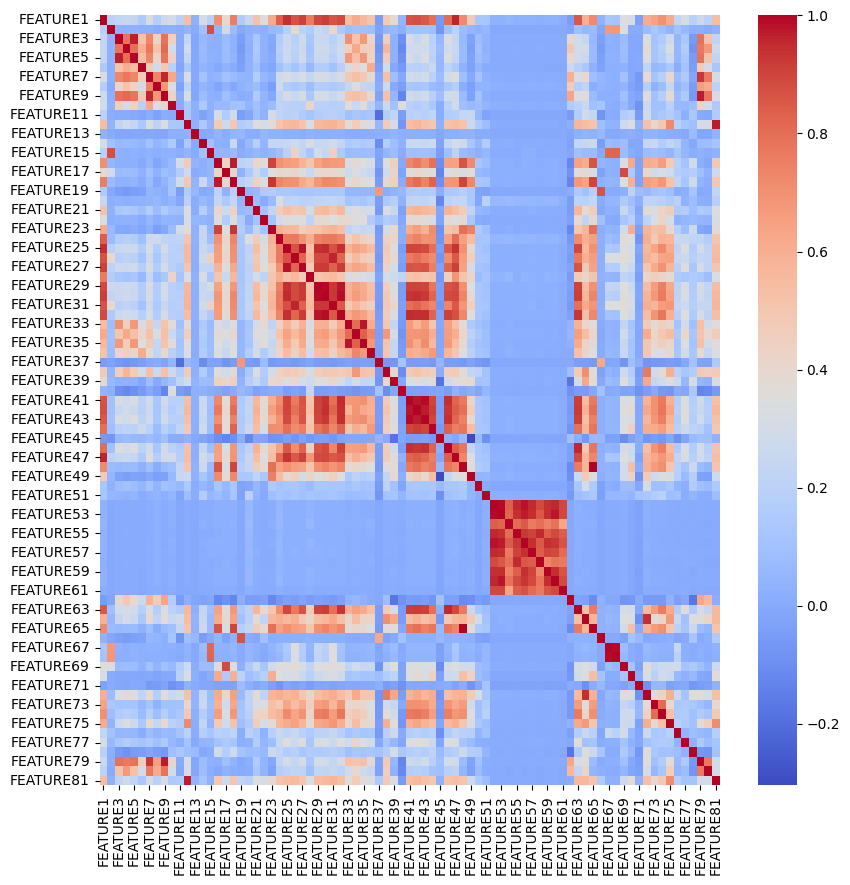
\includegraphics[width=0.8\textwidth]{corr-matrix.png}
        \caption{ماتریس همبستگی میان ویژگی‌ها}
        \label{fig:fig4}
    \end{figure}
    


\newpage
\section{گام چهارم}
این مرحله درواقع مربوط به استفاده از الگوریتم یادگیری بدون ناظر می‌باشد. در دو بخش اول از الگوریتم‌های \lr{K-Means} و \lr{Mini Batch K-Means} استفاده می‌کنیم. و در بخش سوم از الگوریتم \lr{BIRCH} به‌همراه الگوریتم \lr{PCA} به‌منظور کاهش ابعاد داده‌ها استفاده خواهیم کرد.

در این مرحله به‌دلیل حجم بالای داده‌ها با چالش‌های زیادی مواجه شدم. بطور مثال در زیر بخش سوم با ارور \lr{Session crashed. All the RAM was used.} در پروژه \lr{Colab} چندین بار مواجه شدم که مجبور به کاهش ابعاد مدل شدم. و همچنین بدلیل تعداد بالای نمونه‌ها، ارزیابی مدل‌های این مرحله بااستفاده از الگوریتم \lr{Silhoutte} به زمان زیادی احتیاج داشتند.
\subsection{بخش الف)}
در این مرحله ابتدا بااستفاده از تابع  \lr{find\_optimal\_k\_batch()} مقدار بهینه \lr{K} را برای الگوریتم \lr{K-Means} که برروی تمام داده‌ها اجرا خواهد شد، پیدا خواهیم کرد. نحوه ارزیابی مقدار بهینه \lr{K} نیز براساس بیشینه مقدار \lr{Silhoutte} می‌باشد که همانطور که می‌دانیم هرچه به عدد 1 نزدیک‌تر باشد یعنی خوشه‌های بهتری تشکیل شده‌اند. طبق نتایج بدست آمده، مقدار \lr{K = 3} بهترین خروجی را برای ما خواهد داشت. (برای این بخش مقادیر \lr{K} از 2 تا 10 مورد بررسی قرار گرفته‌اند.)
در نهایت الگوریتم \lr{K-Means} با \lr{k = 3} برروی تمامی داده‌ها را مجددا اجرا می‌کنیم. در نهایت در یک حلقه با تعداد دفعات تکرار 81(به تعداد ویژگی‌ها) و محاسبه نسبت بیشینه مسافت درون خوشه و خارج از آن، میزان اهمیت و تاثیرگذاری ویژگی‌ها را محاسبه می‌کنیم.
بخشی از کد مربوط به این بخش را در زیر به‌همراه تعدادی از ویژگی‌ها به‌همراه اهمیتشان می‌توانید مشاهده کنید.

* در فایل اصلی تمامی ویژگی‌ها همراه با میزان اهمیت‌شان آورده‌شده‌اند.
\begin{figure}[ht]
        \centering
        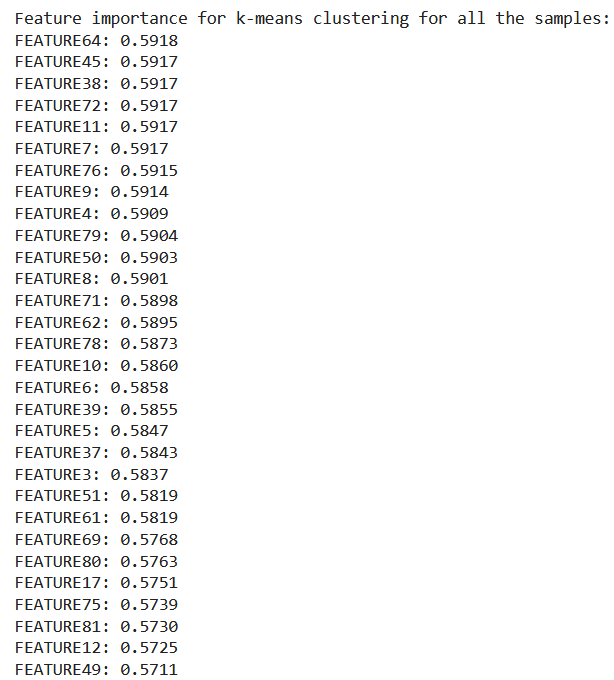
\includegraphics[width=0.7\textwidth]{4-1.png}
        \caption{خروجی بخش 4-الف)}
        \label{fig:fig5}
\end{figure}

\lr{\lstinputlisting[frame=single,
    numbers=left,
    style=Python,
    showstringspaces=false,
    basicstyle=\ttfamily,
    backgroundcolor=\color{gray!20!white},
    breaklines=true]{step4-1.py}}

\newpage
\subsection{بخش ب)}
در این بخش نیز مراحل بخش الف) را تکرار می‌کنیم ولی با این تفاوت که نیاز است الگوریتم \lr{K-Means} را یک بار برروی نمونه‌هایی با برچسب 1 و بار دیگر برروی نمونه‌هایی با برچسب 0 جداگانه اجرا کنیم. در هر بار مقدار بهینه \lr{K} را بااستفاده از معیار \lr{Silhoutte} جداگانه محاسبه کردم. همچنین در نهایت بااستفاده از یک میانگین وزن‌دار نتایج اهمیت ویژگی‌ها را با یکدیگر ادغام کردم.

بخشی از کد مربوط به این بخش را در زیر به‌همراه تعدادی از ویژگی‌ها به‌همراه اهمیتشان می‌توانید مشاهده کنید.

* در فایل اصلی تمامی ویژگی‌ها همراه با میزان اهمیت‌شان آورده‌شده‌اند.

\begin{figure}[ht]
        \centering
        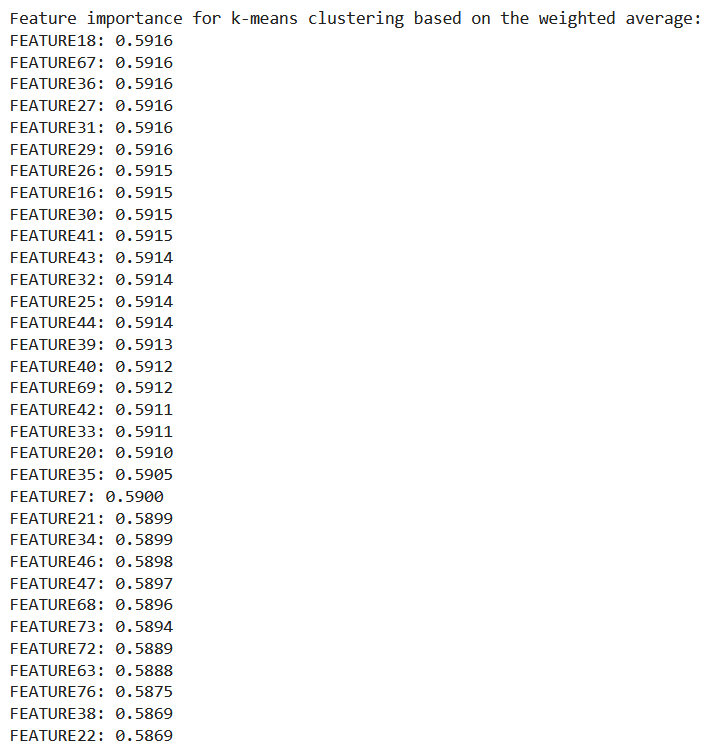
\includegraphics[width=0.7\textwidth]{4-2.png}
        \caption{خروجی بخش 4-ب)}
        \label{fig:fig6}
\end{figure}

\newpage

\lr{\lstinputlisting[frame=single,
    numbers=left,
    style=Python,
    showstringspaces=false,
    basicstyle=\ttfamily,
    backgroundcolor=\color{gray!20!white},
    breaklines=true]{step4-2.py}}


\newpage
\subsection{بخش ج)}
در این مرحله نیز از ما خواسته شده‌است تا با یک الگوریتم خوشه‌بندی دیگر میزان تاثیرگذاری ویژگی‌ها را محاسبه کنیم. ابتدا الگوریتم \lr{Chameleon} را تست کردم. برای این کار طبق توضیحات فرستاده‌شده، سعی کردم از کتابخانه تعریف‌شده یکی از دوستان استفاده کنم. در هنگام استفاده از این الگوریتم به چالش‌هایی همانند نصب کتابخانه‌های مورد نیاز و هماهنگی آن‌ها با سیستم‌عامل مواجه شدم. همچنین پس از رفع مشکلات گفته‌شده به زمانی در حدود 200 ساعت نیاز بود تااینکه داده‌های ورودی را خوشه‌بندی کند.

به‌عنوان جایگزین به‌سراغ استفاده از الگوریتم \lr{DBSCAN} می‌روم. در هنگام استفاده از این الگوریتم حتی با وجود کاهش ابعاد داده‌های ورودی، ولی خطای \lr{Session is crashed.} را در محیط پروژه \lr{Colab} دریافت کردم.

پس از چندین تلاش، در نهایت به‌سراغ استفاده از الگوریتم \lr{BIRCH} رفتم. برای استفاده از این الگوریتم نیز در صورتی که همه داده‌های ورودی را به‌عنوان ورودی استفاده کنیم، خطایی مشابه حالت \lr{DBSCAN} مشاهده خواهیم کرد. در نتیجه در ابتدا بااستفاده از الگوریتم \lr{PCA}، ابعاد داده‌ها را کاهش می‌دهیم. خروجی نهایی مربوط به این الگوریتم و تائیر دو ویژگی اصلی را در تصاویر زیر می‌توانید مشاهده کنید.

\begin{figure}[ht]
        \centering
        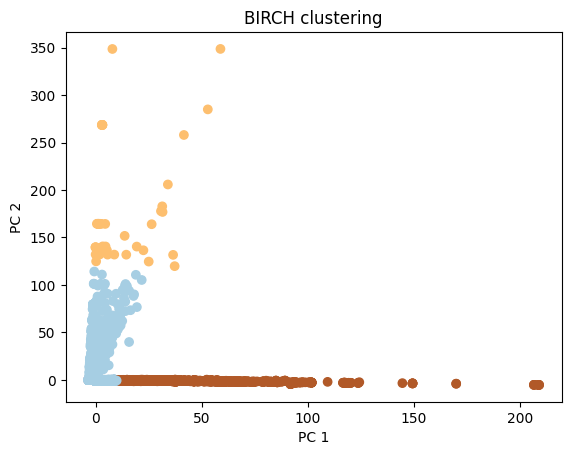
\includegraphics[width=0.6\textwidth]{birch-clus.png}
        \caption{خوشه‌های حاصل از بخش 4-ج)}
        \label{fig:fig7}
\end{figure}

\begin{figure}[ht]
        \centering
        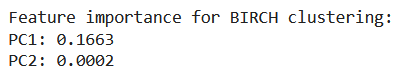
\includegraphics[width=0.6\textwidth]{birch-feature.png}
        \caption{خروجی بخش 4-ج)}
        \label{fig:fig8}
\end{figure}

\newpage
\section{گام پنجم}
در این مرحله باتوجه به خواسته موجود در صورت پروژه الگوریتم \lr{Random Forest} و \lr{XGBoost} جهت یادگیری با نظارت استفاده می‌کنیم. همچنین باتوجه به توزیع نامتقارن داده‌ها با برچسب‌های 0 و 1 در هنگام استفاده از هر یک از الگوریتم‌های ذکر شده، از دو روش برای بهبود نتایج استفاده می‌کنیم.
باتوجه به اینکه بهترین نتایج در حالت \lr{Random Forest with Oversampling} و \lr{Standard XGBoost} بدست می‌آیند، تنها برای این دو حالت تاثیرگذاری و میزان اهمیت هر یک از ویژگی‌ها را محاسبه می‌کنیم.

نتایج گفته‌شده را در تصاویر زیر می‌توانید مشاهده کنید.
\begin{figure}[ht]
        \centering
        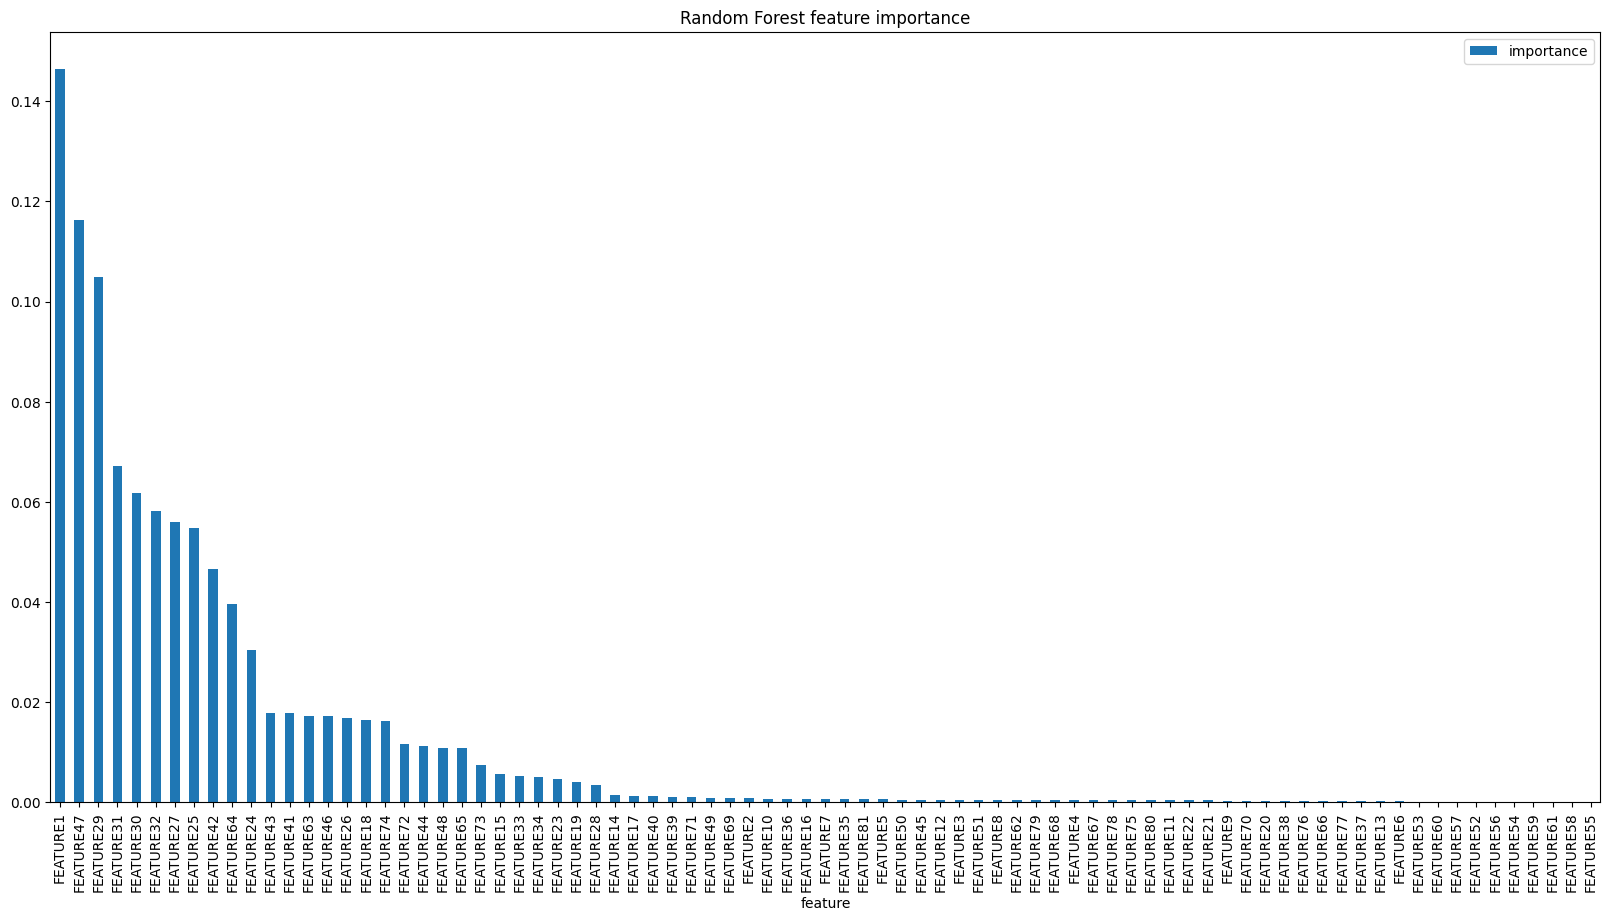
\includegraphics[width=0.75\textwidth]{random-forest-smote-importance.png}
        \caption{میزان اهمیت و تاثیرگذاری ویژگی‌ها برروی الگوریتم \lr{Random Forest with SMOTE}}
        \label{fig:fig9}
\end{figure}

\begin{figure}[ht]
        \centering
        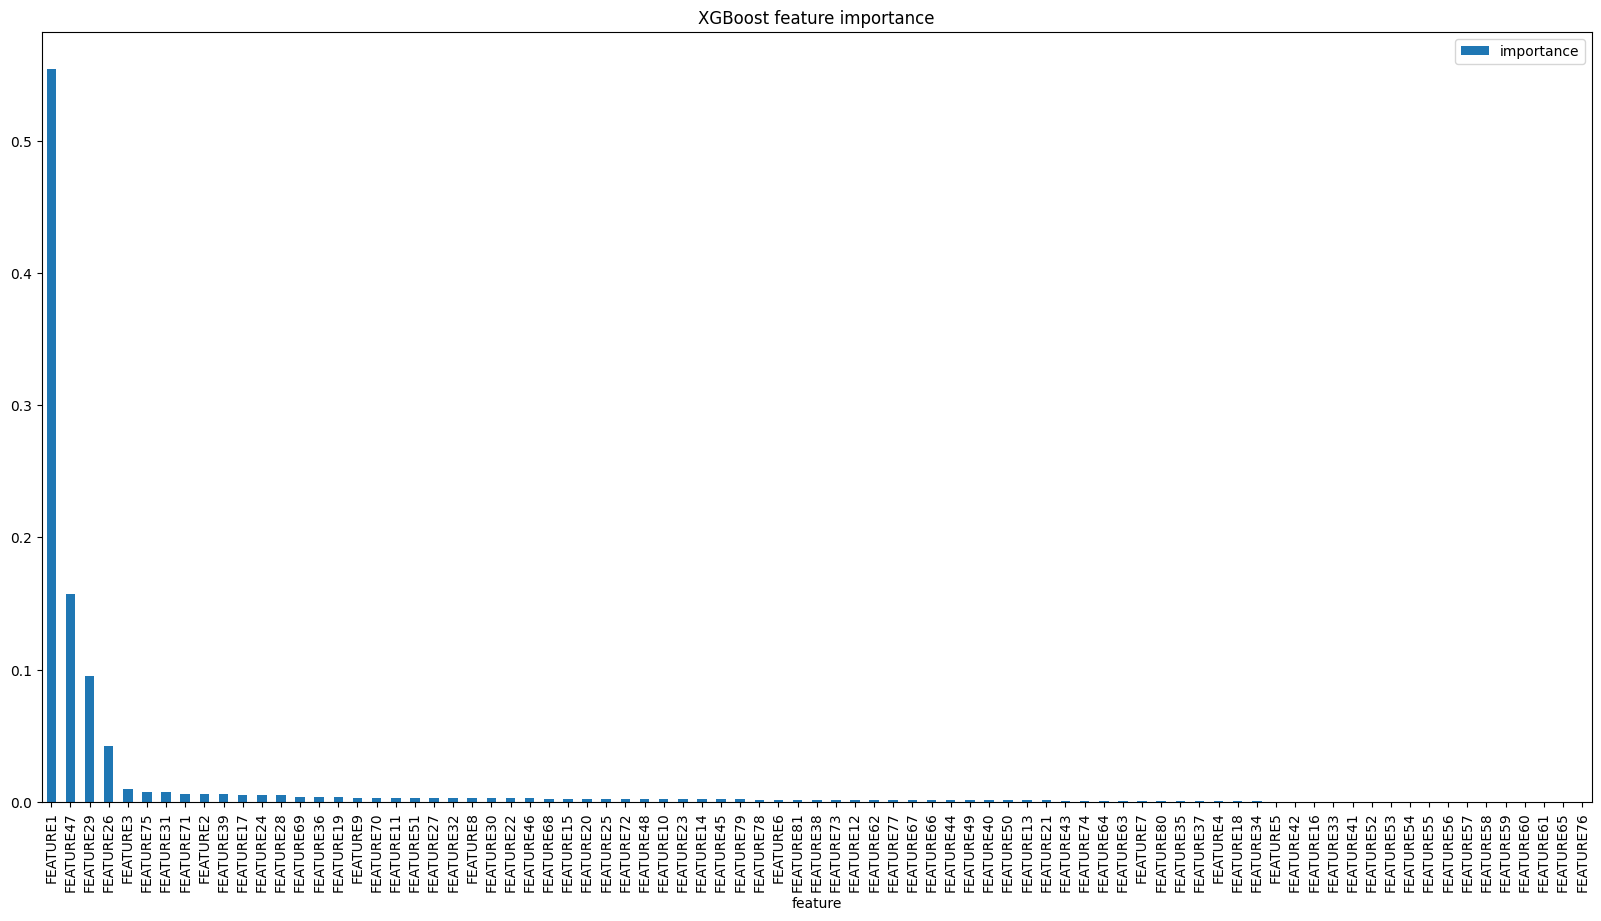
\includegraphics[width=0.75\textwidth]{standard-xgboost-importance.png}
        \caption{میزان اهمیت و تاثیرگذاری ویژگی‌ها برروی الگوریتم \lr{Standard XGBoost}}
        \label{fig:fig10}
\end{figure}

\newpage
\section{گام ششم}
نتایج حاصل از ارزیابی معیارهای گوناگون برروی مدل‌‌های استفاده‌شده را در فایل اکسل ارسال‌شده می‌توانید مشاهده کنید.

همچنین در تصاویر زیر نیز می‌توانید \lr{Confusion Matrix} الگوریتم‌های یادگیری با نظارت استفاده‌شده در حالت‌های مختلف را مشاهده کنید.
\begin{figure}[ht]
    \centering
    \begin{subfigure}[b]{0.36\textwidth}
        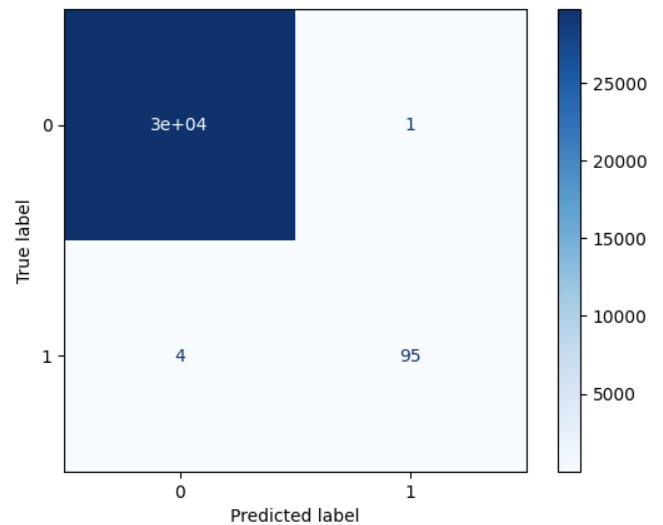
\includegraphics[width=\textwidth]{standard-rf-cm.png}
        \caption{\lr{Standard Random Forest}}
        \label{fig:fig11}
    \end{subfigure}
    \begin{subfigure}[b]{0.36\textwidth}
        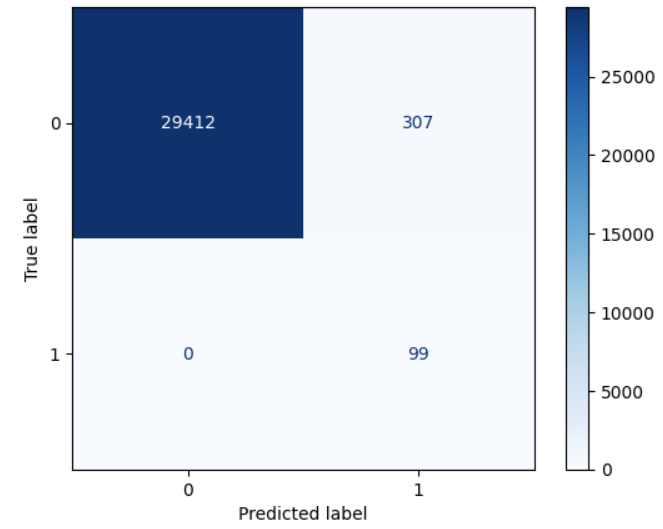
\includegraphics[width=\textwidth]{balanced-rf-cm.png}
        \caption{\lr{Balanced Random Forest}}
        \label{fig:fig12}
    \end{subfigure}
    
    \begin{subfigure}[b]{0.36\textwidth}
        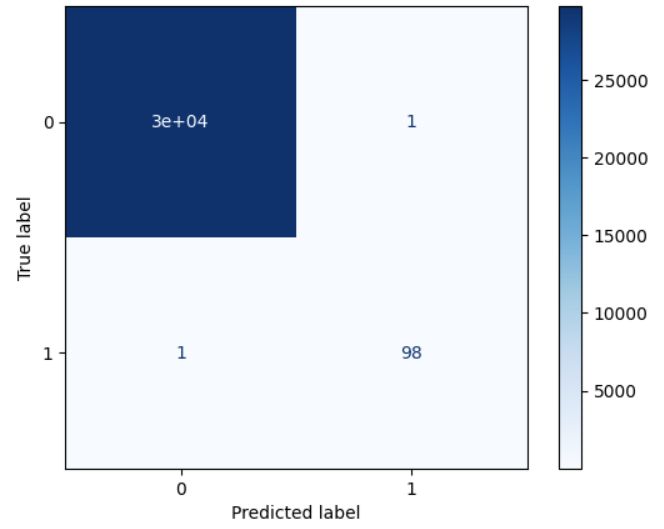
\includegraphics[width=\textwidth]{smot-rf-cm.png}
        \caption{\lr{SMOTE Random Forest}}
        \label{fig:fig13}
    \end{subfigure}
    \begin{subfigure}[b]{0.36\textwidth}
        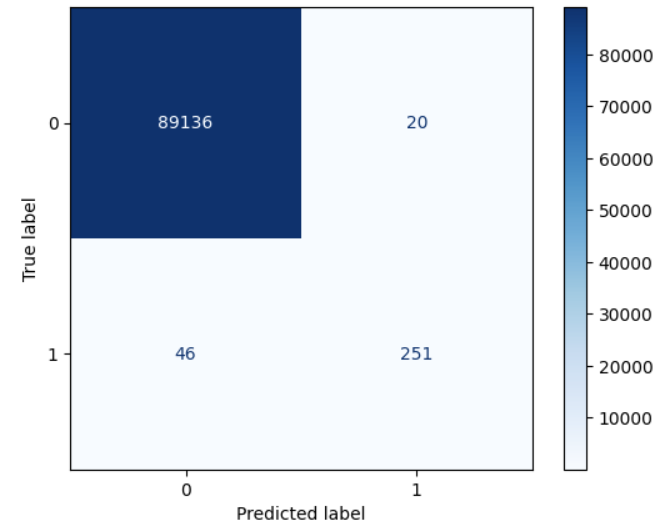
\includegraphics[width=\textwidth]{standard-xgboost-cm.png}
        \caption{\lr{Standard XGBoost}}
        \label{fig:fig14}
    \end{subfigure}

    \begin{subfigure}[b]{0.36\textwidth}
        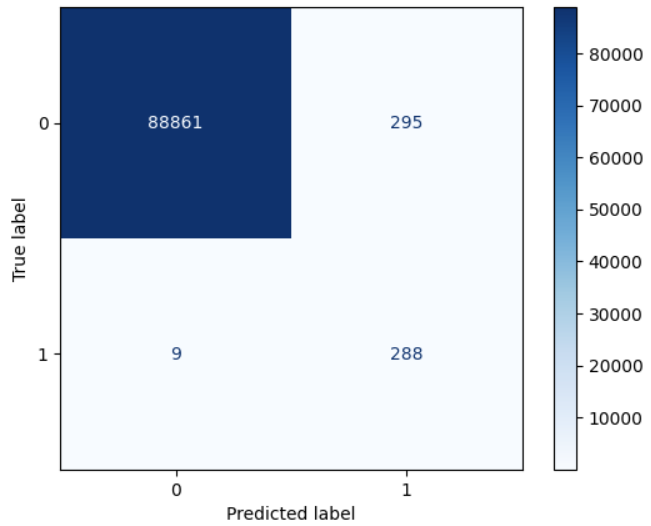
\includegraphics[width=\textwidth]{weighted-xgboost-cm.png}
        \caption{\lr{Weighted XGBoost}}
        \label{fig:fig15}
    \end{subfigure}
    \begin{subfigure}[b]{0.36\textwidth}
        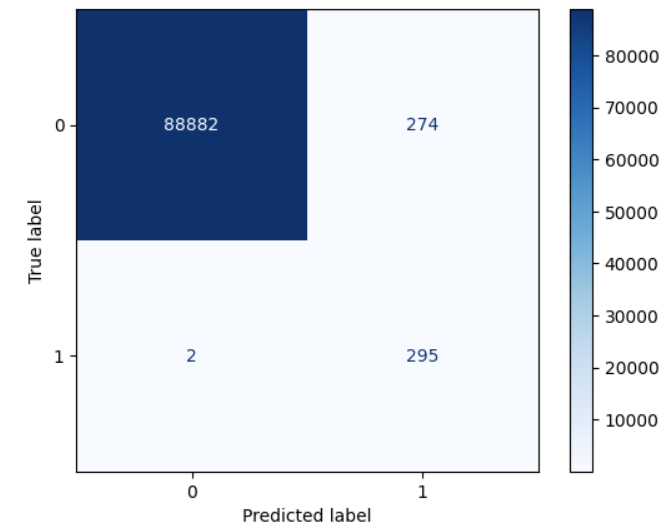
\includegraphics[width=\textwidth]{xgboost-smote-cm.png}
        \caption{\lr{SMOTE XGBoost}}
        \label{fig:fig16}
    \end{subfigure}
\end{figure}

\newpage
\section{نتیجه‌گیری}
\subsection{آیا ویژگی‌هایی وجود دارند که در هر دو نوع یادگیری \lr{Supervised} و \lr{Unsupervised} از نظر تاثیرگذاری هم‌پوشانی داشته باشند؟}
در حالت یادگیری بدون ناظر هم‌پوشانی مشاهده نمی‌شود. ولی در یادگیری باناظر همان‌گونه که در تصاویر گام پنجم توضیح داده شده‌است، اولین ویژگی بیشترین تاثیر در حالت‌های محاسبه‌شده را داشته‌است و بین سایر ویژگی‌ها نیز هم‌پوشانی و شباهت دیده می‌شود.
\subsection{به نظر شما کدام یک از رتبه‌بندی‌ها منطقی‌تر است؟}
باتوجه به نتایج خروجی و همچنین چالش‌های حل مسئله، الگوریتم با ناظر عملکرد بهتری داشته‌اند. باتوجه به‌ حجم بالای داده‌ها در هنگام استفاده از الگوریتم‌های بدون ناظر ممکن است با چالش‌های سخت‌افزاری مواجه شویم. ولی با تغییرات جزئی در الگوریتم‌های با ناظر می‌توانیم به دقت و صحت بالایی دست پیدا کنیم.

همچنین یکی از چالش‌های دیگر در هنگام استفاده از الگوریتم بدون ناظر تعیین مقادیر برای پارامترهای مورد نیاز آن‌ها می‌باشد که نتایج نهایی را تحت تاثیر قرار می‌دهند.
\subsection{اگر اختلاف زیادی در معیارهای ارزیابی روش‌ها مشاهده شد، دلیل آن را بنویسید.}
در الگوریتم‌های با ناظر مقادیر \lr{accuracy}، \lr{precision}، \lr{recall} و \lr{F1-score} شباهت زیادی با یکدیگر دارند.
در حالت استفاده از الگوریتم‌های بی‌ناظر همانطور که در بخش چهار اشاره شده‌است، مقادیر \lr{Silhoutte} شباهت زیادی به یک‌دیگر دارند.
\newpage
\end{document}
